\begin{activity} \label{A:5.1.1}  Suppose that the function $y = f(x)$ is given by the graph shown in Figure~\ref{F:5.1.Act1}, and that the pieces of $f$ are either portions of lines or portions of circles.  In addition, let $F$ be an antiderivative of $f$ and say that $F(0) = -1$.  Finally, assume that for $x \le 0$ and $x \ge 7$, $f(x) = 0$.
\begin{figure}[h]
\begin{center}
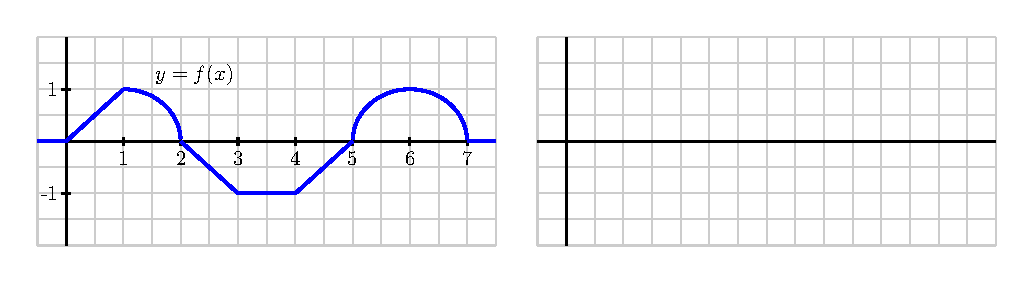
\includegraphics{figures/5_1_Act1.eps}
\end{center}
\caption{At left, the graph of $y = f(x)$.} \label{F:5.1.Act1}
\end{figure}
\ba
	\item On what interval(s) is $F$ an increasing function?  On what intervals is $F$ decreasing?
	\item On what interval(s) is $F$ concave up?  concave down? neither?
	\item At what point(s) does $F$ have a relative minimum?  a relative maximum?
	\item Use the given information to determine the exact value of $F(x)$ for $x = 1, 2, \ldots, 7$.  In addition, what are the values of $F(-1)$ and $F(8)$?
	\item Based on your responses to all of the preceding questions, sketch a complete and accurate graph of $y = F(x)$ on the axes provided, being sure to indicate the behavior of $F$ for $x < 0$ and $x > 7$.  Clearly indicate the scale on the vertical and horizontal axes of your graph.
	\item What happens if we change one key piece of information:  in particular, say that $G$ is an antiderivative of $f$ and $G(0) = 0$.  How (if at all) would your answers to the preceding questions change?  Sketch a graph of $G$ on the same axes as the graph of $F$ you constructed in (e).
\ea
\end{activity}
\begin{smallhint}
\ba
	\item Consider the sign of $F' = f$.
	\item Consider the sign of $F'' = f'$.
	\item Where does $F' = f$ change sign?
	\item Recall that $F(1) = F(0) + \int_0^1 f(t) \, dt$.
	\item Use the function values found in (d) and the earlier information regarding the shape of $F$.
	\item Note that $G(1) = G(0) + \int_0^1 f(t) \, dt$. 
\ea
\end{smallhint}
\begin{bighint}
\ba
	\item Consider the sign of $F' = f$ and recall that wherever $F' > 0$, $F$ is increasing.
	\item Consider the sign of $F'' = f'$ and recall that wherever $F''>0$, $F$ is concave up.  Note particularly that $F''>0$ if and only if $f$ is increasing.
	\item Where does $F' = f$ change sign?  A relative maximum for $F$ will occur wherever $F'$ changes from positive to negative.
	\item Recall that $F(1) = F(0) + \int_0^1 f(t) \, dt$.  Similarly, $F(2) = F(0) + \int_0^1 f(t) \, dt$.
	\item Use the function values found in (d) and the earlier information regarding the shape of $F$.
	\item Note that $G(1) = G(0) + \int_0^1 f(t) \, dt$.  Since $G(0) = 0$ (while $F(0) = -1$), this changes each response in (e) by the same constant amount.
\ea
\end{bighint}
\begin{activitySolution}
\ba
	\item Wherever $F' > 0$, $F$ is increasing, so $F$ is increasing on $(0,2)$ and $(5,7)$, while $F$ is decreasing on $(2,5)$.
	\item Wherever $F''>0$, $F$ is concave up; note particularly that $F''>0$ if and only if $f$ is increasing.  Thus, $F$ is concave up on $(0,1)$, $(4,6)$, and concave down on $(1,3)$, $(6,7)$, and neither on $(3,4)$.
	\item A relative maximum for $F$ will occur wherever $F'$ changes from positive to negative, and thus at $x = 2$; similarly, $F$ has a relative minimum at $x = 5$.
	\item Recall that $F(1) = F(0) + \int_0^1 f(t) \, dt$, so $F(1) = -1 + \frac{1}{2} = -\frac{1}{2}$.  Similarly, $F(2) = F(0) + \int_0^1 f(t) \, dt = -1 + \frac{1}{2} + \frac{\pi}{4} = \frac{\pi}{4} - \frac{1}{2}$.  Continuing these calculations, $F(3) = \frac{\pi}{4} - 1$, $F(4) = \frac{\pi}{4}-2$, $F(5) = \frac{\pi}{4} - \frac{5}{2}$, $F(6) = \frac{\pi}{2} - \frac{5}{2}$,  $F(7) = \frac{3\pi}{4} - \frac{5}{2}$.  Furthermore, since $f(t) = 0$ for all $t < 0$ and all $t > 7$, it follows $F(8) =  \frac{3\pi}{4} - \frac{5}{2}$ and $F(-1) = -1$.
	\item Use the function values found in (d) and the earlier information regarding the shape of $F$.
	\item Note that $G(1) = G(0) + \int_0^1 f(t) \, dt$.  Since $G(0) = 0$ (while $F(0) = -1$), this changes each response in by 1: $G(x) = F(x) + 1$.
\ea
\end{activitySolution}
\aftera